\section{Sistema Embarcado - \emph{Firmware}}
\label{sec:sistema_embarcado}
% Falar sobre como foi feito a divisão das atividades no microcontrolador
% Mostrar ilustração dessa divisão, para ter-se uma visão global das rotinas e suas relações de dependência

A implementação em software embarcado do sistema proposto é dividida em quatro rotinas principais, sendo elas: rotina de comunicação, rotina de calibração, rotina de leitura dos sensores  e a rotina de controle. 
Este trabalho fez uso dos múltiplos \emph{cores} presentes no ESP32. 
O núcleo 1 (também denominado por \emph{APP CPU}) é responsável única e
exclusivamente  pela execução do ciclo de controle que atua em ambos os motores (direito e esquerdo). 
As demais rotinas são executadas de forma concorrente no núcleo 0 (\emph{PRO CPU}), sendo que as rotinas de leitura dos sensores possuem máxima prioridade e a de comunicação possui uma prioridade inferior. Foram realizados testes de tal forma a comprovar que o microcontrolador consegue lidar com essa 
divisão de tarefas sem que ocorra monopolização de recursos por parte de alguma das rotinas, ou seja, o ESP32 (mesmo configurado para a menor frequência de operação, 80 MHz) consegue lidar com as altas taxas de acionamento das rotinas/interrupções. 


\begin{figure}[H]
    \centering
    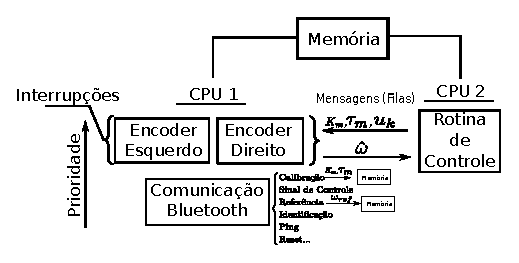
\includegraphics[width=0.7\textwidth]{figuras/ilustracoes/visao_geral_do_sistema.eps}
    \caption{Ilustração do sistema embarcado como um todo.}
    \label{fig:organizacao_firmware}
\end{figure}

A Figura \ref{fig:organizacao_firmware} apresenta uma visão do sistema como um todo. A seguir são apresentadas com mais detalhes cada uma das rotinas presentes no sistema embarcado.

\subsection{Rotina de Comunicação}
\label{subsec:rotina_comunicacao}
% TODO:
% IDEIA: ILUSTRAR A INTERAÇÃO ENTRE A ROTINA PRINCIPAL E A INTERRUPÇÃO
A rotina de comunicação opera em um \emph{loop} infinito no núcleo principal do microcontrolador e é responsável por tratar os telecomandos recebidos pelo \textit{Bluetooth}. Ao ser identificado um recebimento de mensagem pela sinal de interrupção da comunicação \textit{Bluetooth} é acionado a função de tratamento de interrupção correspondente que possui como única função encaminhar as mensagens válida (verificar cabeçalho) para a rotina principal de comunicação. Isso é feito para evitar sobrecarregar a interrupção (podendo atrapalhar as interrupções dos \emph{Encoders} devido a alta prioridade da interrupção).\\

Na rotina principal a mensagem é interpretada e caso ela seja identificado um telecomando válido, será executado a devida resposta, conforme apresentado mais adiante.

O protocolo implementado foi pensado para conter até três campos básicos, o \textbf{\textit{Header}} com 4 bits (servindo de preambulo), para ajudar a sincronizar os pacotes, o identificador de comando \textbf{\textit{CMD}} também com 4 bits, possibilitando assim até 16 comandos distintos e por fim, o campos de argumentos com tamanho variável. Foram implementados 7 comandos.

% Please add the following required packages to your document preamble:
% \usepackage[table,xcdraw]{xcolor}
% If you use beamer only pass "xcolor=table" option, i.e. \documentclass[xcolor=table]{beamer}
\begin{table}[H]
\centering
\begin{tabular}{c|r}
\hline
\rowcolor[HTML]{C0C0C0} 
\multicolumn{1}{|c|}{\cellcolor[HTML]{C0C0C0}DEFINIÇÕES} & \multicolumn{1}{r|}{\cellcolor[HTML]{C0C0C0}VALOR(HEX)} \\ \hline
HEAD & A0 \\
\rowcolor[HTML]{EFEFEF} 
CMD\_REQ\_CAL & 00 \\
CMD\_REQ\_OMEGA & 03 \\
\rowcolor[HTML]{EFEFEF} 
CMD\_CALIBRATION & 04 \\
CMD\_IDENTIFY & 05 \\
\rowcolor[HTML]{EFEFEF} 
CMD\_SET\_POINT & 0A \\
CMD\_CONTROL\_SIGNAL & 0B \\
\rowcolor[HTML]{EFEFEF} 
CMD\_PING & 0F
\end{tabular}
\caption{Definições utilizadas.}
\label{tab:defines}
\end{table}

A Tabela \ref{tab:defines} apresenta as definições/nomenclaturas utilizadas nas descrições a seguir.

\textbf{Comandos}
\begin{itemize}
    \item \textbf{CMD\_REQ\_CAL}:\\
        \textit{Host} envia, para solicitar os dados provenientes da calibração do controlador \textit{Feedforward}. O escravo (robô) envia 4 \emph{Floats}, referente aos coeficientes do controlador.
    \item \textbf{CMD\_REQ\_OMEGA}:\\
        \textit{Host} envia, para solicitar as velocidades atuais de ambos os motores, em $rad/s$. O escravo responde com dois \emph{Floats}, referentes aos ômegas em cada motor.
    \item \textbf{CMD\_CALIBRATION}:\\
        \textit{Host} envia, para fazer com que o robô inicie sua rotina de calibração do controlador.
    \item \textbf{CMD\_IDENTIFY}:\\
        \textit{Host} envia, fazendo com que o robô inicia sua rotina de identificação (rotina que armazena as velocidades durante um certo período de tempo e envia para o \emph{Host}, útil para testes). O \textit{Host} deve enviar o \emph{Bitstream} da seguinte forma:\\
        
        % Please add the following required packages to your document preamble:
% \usepackage{graphicx}
% \usepackage[table,xcdraw]{xcolor}
% If you use beamer only pass "xcolor=table" option, i.e. \documentclass[xcolor=table]{beamer}
\begin{table}[H]
\centering
\resizebox{\textwidth}{!}{%
\begin{tabular}{|
>{\columncolor[HTML]{C0C0C0}}l |
>{\columncolor[HTML]{C0C0C0}}l |l|l|l|}
\hline
HEAD & CMD\_IDENTIFY & OPTIONS & SETPOINT & STEPTIME \\ \hline
\end{tabular}%
}
\end{table}
        
        Sendo o campos \textbf{Options} de 1 byte, contendo a informação de qual motor será feita a identificação e se deve ser usado o controlador.
        
        Ao concluir a rotina de identificação, o robô responde enviando o vetor de ômegas medidos, durante a rotina, para o \textit{Host}, que deve estar aguardando recebê-las. A quantidade de dados será $(timeout/steptime)*4$ bytes, portando o \textit{Host} deve estar aguardando exatamente essa quantidade de bytes.
        
        
    \item \textbf{CMD\_SET\_POINT}:\\
        
        % Please add the following required packages to your document preamble:
% \usepackage{graphicx}
% \usepackage[table,xcdraw]{xcolor}
% If you use beamer only pass "xcolor=table" option, i.e. \documentclass[xcolor=table]{beamer}
\begin{table}[H]
\centering
\resizebox{\textwidth}{!}{%
\begin{tabular}{|
>{\columncolor[HTML]{C0C0C0}}c |
>{\columncolor[HTML]{C0C0C0}}c |c|c|c|c|l|l|l|}
\hline
HEAD & CMD\_SET\_POINT & SENSE\_L & OMEGA\_L & SENSE\_R & \multicolumn{4}{c|}{OMEGA\_R} \\ \hline
\end{tabular}%
}

\end{table}
        
        Neste os campos de \textbf{Sense\_x} indicam o sentido de rotação do motor, 0 para trás e 1 para rodar para frente (convertidos em sinal dos ômegas de Set-point), portando só ocupam 1 bit, já os campos referentes aos ômegas desejados ocupam 15 bits, sendo assim é possível enviar referências com uma precisão de $1.0/2^{15}$, já que as referências serão enviadas inteiras  (0 - $2^{15}$) e mapeadas de $-1.0$ a $1.0$, indicando uma porcentagem da referência da velocidade máxima do robô. Ou seja os campos referentes aos \textit{Set-points} contêm a porcentagem da velocidade máxima do robô.
        
    \item \textbf{CMD\_CONTROL\_SIGNAL}:\\
        
        O comando difere apenas o campo de \textbf{CMD} do comando anterior. O restante da estrutura é exatamente igual, pois a principal diferença ocorre no microcontrolador. Em vez dos campos referentes aos ômegas serem porcentagens da velocidade máxima que será convertido em \textit{Set-point} para o controlador, neste comando o robô irá interpretar esses campos como sendo sinais de controle (após convertê-los para \emph{Float} de $-1.0$ a $1.0$).
        
    \item \textbf{CMD\_PING}:\\
        Neste comando o \textit{Host} pode enviar qualquer mensagem no campo de argumentos, pois o robô irá apenas responder com a mesma mensagem. Este comando é útil para testar conexão e testar a latência da conexão.
    
\end{itemize}
\subsection{Rotina de Calibração}
\label{subsec:rotina_calibracao}

Rotina responsável por realizar a identificação dos parâmetros do modelo dos motores direito e esquerdo do robô: constante de tempo; ganho de malha aberta; parâmetros do controlador \emph{FeedForward}; velocidade máxima de cada motor. Bem como calcular os ganhos para o controlador \emph{P} de forma a se obter uma resposta pré-definida em malha fechada.\\

A rotina de calibração consiste em três etapas que são repetidas para todas as configurações: motor direito para frente; motor direito para trás; motor esquerdo para frente e motor esquerdo para trás. Cada etapa é descrita a seguir: \\

% TO DO:
% ORGANIZAR E REPENSAR A FORMA DE EXIBIR AS ETAPAS
% FIGURAS ILUSTRANDO O COMPORTAMENTO GERAL DAS FUNÇÕES QUE ESTÃO SENDO USADAS NA INTERPOLAÇÃO
% PSEUDO CÓDIGOS TALVEZ

\textbf{ETAPA 1.} Estimar a zona morta e o ganho da planta em malha aberta. Para isso é realizado a coleta de $N$ pontos ($\omega$,$u$), o primeiro ponto é coletado para $u = \pm1$(valor máximo no sentido de giro atual) e são realizados sucessivos decréscimos neste valor até a parada do motor ($\omega = 0$). A aquisição destes pontos ocorre da maior velocidade para a menor, pois a zona morta será mais baixa neste sentido, devido à inércia do motor.\\

Ao se encerrar a coleta destes pontos ($\omega_{ss} = 0$ detectado) é realizado uma regressão linear por mínimos quadrados, tendo $u$ no eixo das ordenadas e $\omega$ no eixo das abscisas, o coeficiente angular dessa reta relaciona a velocidade angular ($\omega$) com o sinal de controle ($u$), já o coeficiente linear representa a zona morta, ou seja, o menor $\omega$ que pode iniciar o giro do motor (\emph{Dead Zone ($D$)}). A regressão linear é possível, apesar do comportamento não linear (como também explorado em \cite{dead_zone}) entre a velocidade e o sinal de controle e ilustrado na Figura \ref{fig:ilustracao_omega_x_pwm}, se analisado um sentido de rotação por vez.

\begin{equation}
    \omega_{ss}(u) = \alpha(u + D)
    % u(\omega) = a\omega + b
    \label{eq:omega_x_sinal_de_controle}
\end{equation}

Com os parâmetros dessa reta (Equação \ref{eq:omega_x_sinal_de_controle}) é possível estimar o ganho de malha aberta da planta da seguinte forma:

\begin{equation}
    K_m = \alpha(u_{max} + D)
    % K_m = \frac{(u_{max} - b)}{a}
\end{equation}

A Figura \ref{fig:ilustracao_omega_x_pwm} apresenta uma ilustração da relação entre o \emph{PWM} (sinal de controle) e a velocidade de regime $\omega_{ss}$ do motor.

\begin{figure}[H]
    \centering
    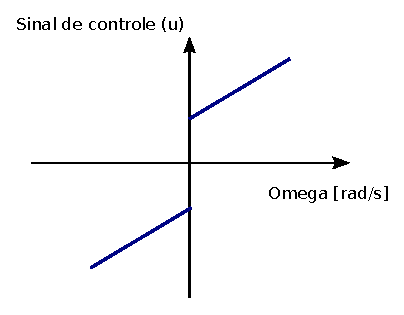
\includegraphics[width=0.5\textwidth]{figuras/ilustracoes/omega_x_sinal_controle.eps}
    \caption{Comportamento da curva $\omega_{ss}(u)$.}
    \label{fig:ilustracao_omega_x_pwm}
    \fonte{Própria.}
\end{figure}

    
\textbf{ETAPA 2.} Estimar a constante de tempo. Para obter a constante de tempo da planta na configuração atual, faz-se uso mais uma vez de interpolação por \textit{MMQ} e tira-se proveito do conhecimento do ganho da planta para simplificar e tornar possível essa interpolação de forma simples. Para estimar a constante de tempo obtém-se $M$ pontos ($t$,$\omega$) e aplica-se o \textit{MMQ} para uma interpolação linear, para isso é necessário fazer a seguinte alteração:
    

\begin{align*}
    \omega(t) &= K\left( 1 - e^{-t/T_m} \right)\\
    \ln{\omega(t)} &= \ln\left[K( 1 - e^{-t/T_m})\right]\\
    \ln\left(1 - \frac{\omega(t)}{K} \right) &= -\frac{t}{T_m}\\
    y_{aux}(t) &= -\frac{t}{T_m}
\end{align*}

Convertendo $\omega(t)$ para $y_{aux}(t)$ o coeficiente angular resultante da interpolação linear será: $coef.angular = -\frac{1}{T_m}$, dessa forma obtemos a constante de tempo.\\

\textbf{ETAPA 3.} Calcular os parâmetros do controlador \textit{Feedback}. O ganho do controlador proporcional se relaciona com o polo (inverso do negativo da constante de tempo desejada) desejado para o sistema em malha fechada, por meio da relação \ref{eq:calculo_do_Kp}. Esse cálculo só é possível devido à identificação dos parâmetros da planta resultante das etapas anteriores. O polo desejado para todas as configurações da planta é uma constante pré-definida, que para os experimentos apresentados neste trabalho foi de $-20$ (equivalente a um $\tau_m$ desejado de 0.08s).\\

\begin{equation}
    K_p = -\frac{\tau_m S_d + 1}{K_m}
    \label{eq:calculo_do_Kp}
\end{equation}

Sendo $S_d$ o polo desejado para o sistema em malha fechada, que é equivalente à $S_d = -1/\tau_{m_{d}}$.
    

Ao se passar por todas as configurações de motor/sentido a rotina seleciona a menor das velocidades máximas apresentada por alguma dessas configurações e armazena esta velocidade como sendo a velocidade máxima atingida pelos motores deste robô (na prática é armazenado 90\% desse valor, para dar uma margem de factibilidade), isso é importante, para assegurar que a referencia $\omega_{ref}$ seja factível para todas as configurações. \\

Por fim os resultados são armazenados na memória permanente do microcontrolador, sendo atualizado/sobrescritos apenas ao final da próxima chamada da rotina de calibração.
\subsection{Rotina de Leitura dos Sensores}
\label{subsec:rotina_sensores}
% TODO:
% REALIZAR ANÁLISE DE FREQ. MÁXIMA DE OPERAÇÃO DOS ENCODERS VS BANDA DISPONIVEL NAS INTERRUPÇÕES RESPONSAVEIS PELA LEITURA DOS ENCODERS

Há duas interrupções associadas aos sinais provenientes dos \emph{Encoders} rotativos, uma para cada motor, cujo objetivo é medir a velocidade de rotação do eixo do motor ($\omega_{medido}$) bem como aplicar o filtro de \emph{Kalman} para uma melhor estimativa da mesma ($\hat{\omega}$). As interrupções são provocadas pelas bordas dos pulsos de ambos os canais, fazendo com que a resolução do sensor seja utilizada ao máximo, pois dessa maneira os sensores que possuem uma resolução de três pulsos por revolução (em cada canal, ver Figura \ref{fig:ilustracao_uma_revolucao}) consigam acionar doze (12) vezes a interrupção que irá computar o $\omega_{motor}$, passando assim a ser ter uma resolução equivalente a doze pulsos por revolução.\\

Para o cálculo do módulo da velocidade de rotação do eixo do motor faz-se uso da medição pelo período do sinal (conforme a Equação \ref{eq:omega_periodimetro}) com os seguintes parâmetros:

\begin{itemize}
    \item $N_{PR} = 12$. Pois são $12$ interrupções por canal (monitorando ambas as bordas de subida e descida de um dos canais);
    \item $T_{hf} = 1\mu{}s$. O contador de alta precisão do $ESP32$ possui, idealmente, uma resolução de $1\mu{}s$ \cite{esp}.
\end{itemize}

A escolha do método de leitura por periodímetro em vez do frequencímetro se deu devido assim ser possível a leitura imediata da velocidade, pois basta apenas uma interrupção para se ter uma medição e também devido à boa precisão da leitura para baixas velocidades, mesmo que isso piore para altas velocidades (como mostrado na Equação \ref{eq:erro_quantizacao_periodimetro}).

\begin{figure}[H]
    \centering
    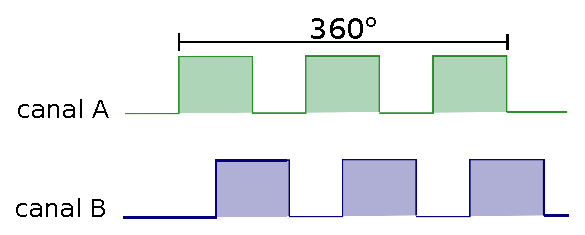
\includegraphics[width=0.5\textwidth]{figuras/ilustracoes/sinal_enquadratura_uma_revolucao.eps}
    \caption{Ilustração do sinal em quadratura em uma revolução completa do eixo do motor no sentido horário.}
    \label{fig:ilustracao_uma_revolucao}
    \fonte{Própria.}
\end{figure}

Já para se obter o sentido de rotação do motor, fez-se uso do padrão \emph{Gray Code} gerado pela diferença de fase entre os diferentes canais de um mesmo sensor. Uma maneira de fazer isso é ler os \emph{GPIO}'s associados aos canais do \emph{Encoder} e verificar o padrão em binário e inferir o sentido de rotação (conforme apresentado na \autoref{sec:encoders}). Porém esse procedimento apresentou uma alta taxa de erro na inferência do sentido para médias e altas velocidades. \\

A abordagem adotada aqui foi armazenar os dois \emph{bits}(sendo canal A bit mais significado) e concatenar/somar com os últimos dois \emph{bits} (da leitura anterior) deslocados em dois (equivalente à multiplicar por $2^2$ ou operar bit-a-bit: $bits_{anteriores} << 2$), criando assim um padrão com $4$ \emph{bits}, sendo os dois mais significativos o padrão da leitura anterior e os dois menos significativos a leitura atual. Esse procedimento é ilustrado para uma rotação no sentido horário e no sentido anti-horário respectivamente nas Tabelas \ref{tab:tabela_gray_code_cw} e \ref{tab:tabela_gray_code_ccw}, dessa forma geram-se quatro($4$) padrões/códigos que caracterizam um tipo de rotação. Esse padrão de $4$\emph{bits} é armazenado de forma estática em um vetor(uma tabela de cola/ \emph{Lookup Table}) nas rotinas de ambos os motores. Esse vetor mapeia o código binário em $1$, $-1$ ou zero para as combinações que não caracterizam um sentido de giro. O sinal do valor corresponde ao sentido horário ou anti-horário e depende do motor. Os vetores \emph{lookup table} para ambos os motores são apresentados  nas Tabela \ref{tab:lookup_table_motor_esquerdo} e \ref{tab:lookup_table_motor_direito}.

% Please add the following required packages to your document preamble:
% \usepackage{graphicx}
\begin{table}[H]
\centering
\resizebox{0.5\textwidth}{!}{%
\begin{tabular}{c|c|c|c|c}
\textbf{$A_{ant}$} & \textbf{$B_{ant}$} & \textbf{$A_{atual}$} & \textbf{$B_{atual}$} & \textbf{DEC} \\ \hline
0 & 0 & 1 & 0 & 2 \\
1 & 0 & 1 & 1 & 11 \\
1 & 1 & 0 & 1 & 13 \\
0 & 1 & 0 & 0 & 4
\end{tabular}%
}
\caption{Codificação de 4 \emph{bits} para a rotação no sentido horário.}
\label{tab:tabela_gray_code_cw}
\end{table}
% Please add the following required packages to your document preamble:
% \usepackage{graphicx}
\begin{table}[H]
\centering
\resizebox{0.5\textwidth}{!}{%
\begin{tabular}{c|c|c|c|c}
\textbf{$A_{ant}$} & \textbf{$B_{ant}$} & \textbf{$A_{atual}$} & \textbf{$B_{atual}$} & \textbf{DEC} \\ \hline
0 & 0 & 0 & 1 & 1  \\
0 & 1 & 1 & 1 & 7  \\
1 & 1 & 1 & 0 & 14 \\
1 & 0 & 0 & 0 & 8 
\end{tabular}%
}
\caption{Codificação de 4 \emph{bits} para a rotação no sentido anti-horário.}
\label{tab:tabela_gray_code_ccw}
\end{table}
% Please add the following required packages to your document preamble:
% \usepackage{graphicx}
\begin{table}[H]
\centering
\resizebox{0.8\textwidth}{!}{%
\begin{tabular}{c|ccccllllllllllll}
\textbf{Índice} & 0 & 1  & 2 & 3 & 4 & 5 & 6 & 7  & 8  & 9 & 10 & 11 & 12 & 13 & 14 & 15 \\ \hline
\textbf{Valor}  & 0 & -1 & 1 & 0 & 1 & 0 & 0 & -1 & -1 & 0 & 0  & 1  & 0  & 1  & -1 & 0 
\end{tabular}%
}
\caption{\emph{Lookup table} para o motor esquerdo.}
\label{tab:lookup_table_motor_esquerdo}
\end{table}
% Please add the following required packages to your document preamble:
% \usepackage{graphicx}
\begin{table}[H]
\centering
\resizebox{0.8\textwidth}{!}{%
\begin{tabular}{c|ccccllllllllllll}
\textbf{Índice} & 0 & 1  & 2 & 3 & 4 & 5 & 6 & 7  & 8  & 9 & 10 & 11 & 12 & 13 & 14 & 15 \\ \hline
\textbf{Valor}  & 0 & 1 & -1 & 0 & -1 & 0 & 0 & 1 & 1 & 0 & 0  & -1  & 0  & -1  & 1 & 0 
\end{tabular}%
}
\caption{\emph{Lookup table} para o motor direito.}
\label{tab:lookup_table_motor_direito}
\end{table}

Com a \emph{lookup table} e o módulo da velocidade é possível calcular a velocidade de rotação da seguinte forma:

\begin{equation}
    \omega_{\text{medido}} = \frac{2\pi}{N_{PR}\Delta{t}}\text{table}[\text{code}]
\end{equation}

Sendo,

\begin{equation*}
    \Delta{t} = nT_{hf}
\end{equation*}

Uma vez calculado o $\omega_{medido}$, calcula-se em 
seguida a melhor estimativa para $\omega$ ($\hat{\omega}$) 
utilizando-se o filtro de \emph{Kalman} (conforme apresentado na \autoref{sec:kalman}). 
Para isso é considerado que o sistema $\omega(t)$ possui um comportamento de primeira ordem 
(conforme Equação \ref{eq:motor_transf_func}), fazendo com que as variáveis do filtro sejam:

\begin{equation*}
\begin{cases}
    \textbf{x}_k = \left[ \omega_k \right]\\
    \textbf{z}_k = [\omega_k]\\
    \textbf{F}_k = [1]\\
    \textbf{H}_k = [1]
\end{cases}
\end{equation*}

Considera-se também que os erros de quantização nas observações comportam-se como ruído gaussiano (essa consideração é possível de acordo com \cite{quantization_error_is_a_gaussian}).

Modelo da \textbf{medição}:
\begin{align*}
z_k = \omega_{medido}
\end{align*}

Com isso a etapa de \textbf{predição} do filtro torna-se:
% MUDAR O SIMBOLO QUE FAZ REFERENCIA À ENTRADA (u) DE ENTRADA
\begin{align*}
    \check{\omega}_{k|k-1} &= \hat{\omega}_{k-1} + (u_k.K_m - \hat{\omega}_{k-1})\left( 1 - e^{-\Delta{t}/T_m} \right)\\
    \check{P}_{k|k-1} &= \hat{P}_{k-1} + Q_k
\end{align*}

Sendo $u_k$ o sinal de controle no instante $k$.\\

E a etapa de atualização \textbf{Atualização} é:

\begin{align*}
K_k &= \check{P}_k \left( \check{P}_k + R_k \right)^{-1} = \frac{\check{P}_k}{\check{P}_k + R_k}\\
\hat{\omega}_k &= \check{\omega}_k + K_k \left( \omega_{k_{medido}} - \check{\omega}_k \right)\\
\hat{P}_k &= \left( 1 - K_k \right) \check{P}_k
\end{align*}

Os parâmetros do filtro foram sintonizados experimentalmente, sendo eles:

\begin{itemize}
    \item $Q = 10$;
    \item $R = 1200$, notou-se pouca variação nesse valor da variância da medição (o valor foi obtido calculando-se a variância da resposta da planta/motor em regime permanente).
    \item $P_0 = 60$, valor inicial da incerteza da melhor estimativa.
\end{itemize}

Foram utilizados estruturas do tipo fila (\emph{Queue} de tamanho 1, para não causar atrasos extras) para enviar e receber estruturas de dados entre as interrupções dos sensores e as demais rotinas em execução no ESP32. Dessa maneira foi possível evitar o uso de variáveis globais e permitiu a troca de informação com a rotina de controle que fica em execução em um núcleo diferente do microcontrolador. A fila de saída contém a estimativa da velocidade e a fila de entrada contém os parâmetros do filtro, bem como o último sinal de controle. Um pseudo código ilustrando a rotina de leitura dos sensores é apresentado a seguir:

\begin{algorithm}
\caption{Rotina de Leitura dos Sensores}
\label{alg:rotina_leitura_sensores}
\begin{algorithmic}[1]
  \State $lookup\_table \gets $ \{0, 1, -1, 0, 0, 0, 0, 1, 0, 0, 0, -1, 0, 1, -1, 0\}

  % atualiza o codigo
  \State $code \gets \left(code \ll 2\right)$ 
  \State $code \gets code + \left(\left(READ\_GPIO(CANAL\_A)\ll1\right)+READ\_GPIO(CANAL\_B)\right)$
    
  \Comment{Obtém o tempo atual em segundos.}
  \State $t_1 \gets get\_time()$
  
  \State $\Delta{t} \gets  t_1 - t_0$
  
  \Comment{Atualiza a referência de tempo anterior $t_0$}
  \State $t_0 \gets t_1$
  
  \State $\omega_{medido} \gets \frac{2\pi}{N_{PR}*\Delta{t}}$ * $lookup\_table[code]$
  
  \Comment{Verifica se tem os dados para usar o filtro.}
  \If{ $queue\_input.empty()$ \textbf{E} nunca recebeu}\\
    \Comment{Coloca o $\omega_{medido}$ na fila de saída e encerra a rotina.}
    \State $queue\_output \gets \omega_{medido}$
    \State return;
  \EndIf
  
  \Comment{Caso tenha novos dados (fila de entrada não vazia) atualizar os dados presentes na rotina. Se não usar os dados anteriores.}
  \State $\omega_{ss}$,$\tau$ $\gets  queue\_input$

%   //predição
  \Comment{Etapa de predição.}
  \State $\check{\omega} \gets \omega_{medido}$ + $( \omega_{ss} - \omega_{medido} ) * (1 - exp(-\Delta{t}/\tau))$
  \State $\check{P} \gets \hat{P} + Q$


%   //atualização
  \Comment{Etapa de atualização.}
  \State $K_{gain} \gets \check{P} / (\check{P} + R)$
  \State $\hat{\omega} \gets \check{\omega}$ + $K_{gain} * (\omega_{medido} - \check{\omega})$
  \State $\hat{P} \gets (1 - K_{gain}) * \check{P}$ 
  
  \State $queue\_output \gets \hat{\omega}$
\end{algorithmic}
\end{algorithm}

\subsection{Rotina de Controle}
\label{subsec:rotina_controle}
Para garantir que não ocorram interrupções, o controle é executado sozinho no núcleo secundário (APP CPU) do ESP32. A rotina opera em \emph{loop} infinito com uma taxa de atualização de $5$ ms.\\

Primeiramente a rotina verifica (para cada motor) se existem novas leituras de velocidades, providas pelas interrupções dos sensores. Caso existam, esses valores são atualizados e é passado para a etapa seguinte. Caso contrário é verificado a quanto tempo esses valores não são atualizados. Caso esse tempo seja superior a um limiar pré-definido (no trabalho foi usado esse limiar igual a 500ms) será considerado que o motor-roda em questão está parado ($\hat{\omega} = 0$) e avança-se para a etapa seguinte.\\

Com a informação da velocidade atualizada (ou mantida, caso não tenha havido nova leitura), lê-se as referências para os motores direito e esquerdo. Essas referências inicialmente são valores no intervalo [$-1$, $1$], pois indicam a porcentagem da velocidade que deve ser o \emph{set point} do controlador. \\
% Em seguida calcula-se as referências em rad/s multiplicando-as pela velocidade máxima ($\omega_{max}$) do robô (obtida na etapa de calibração).\\

A etapa seguinte é realizar os cálculos de controle, porém antes disso é necessário converter a referência para $rad/s$, faz-se isso multiplicando as referências relativas (provenientes da comunicação) pela velocidade máxima do robô ($\omega_{max}$), obtida na etapa de calibração. A seguir, são computadas, separadamente, a contribuição do controlador \emph{Feedforward} (conforme \ref{eq:feedforward}) e o proporcional (conforme \ref{eq:proporcional}) para ao final somá-las e assim obter o sinal de controle (PWM/$u(t) \in [-1,1]$). Após o sinal de controle passar por um saturador (para garantir que esteja no intervalo admissível) o sinal PWM para ambos os motores é enviado para o \emph{Driver motor} que tratará de excitar as entradas dos motores com as correspondentes tensões. A Figura \ref{fig:diagrama_de_controle_simplificado} apresenta uma visão geral simplificada do sistema de controle . A Figura \ref{fig:diagrama_sistema_de_controle_feedforward_backward} ilustra o ciclo de controle \emph{Feedforward} + \emph{Backward}.

\begin{equation}
    u_{ff} = \omega_{ref}\alpha + D
    \label{eq:feedforward}
\end{equation}

\begin{equation}
    u_{p} = (\omega_{ref} - \hat{\omega})K_p
    \label{eq:proporcional}
\end{equation}

\begin{figure}[H]
    \centering
    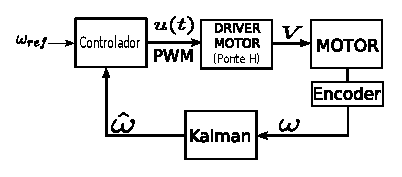
\includegraphics[width=0.5\textwidth]{figuras/ilustracoes/sistema_de_controle_embarcado.eps}
    \caption{Diagrama simplificado do ciclo de controle.}
    \label{fig:diagrama_de_controle_simplificado}
    \fonte{Própria.}
\end{figure}

\begin{figure}[H]
    \centering
    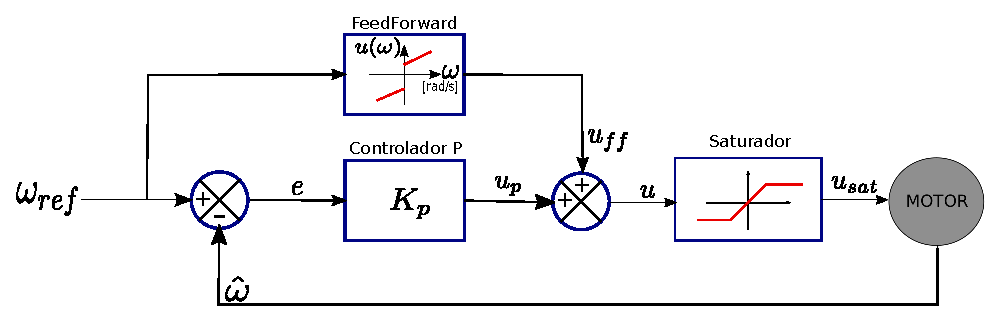
\includegraphics[width=\textwidth]{figuras/ilustracoes/sistema_de_controle_completo.eps}
    \caption{Diagrama de um sistema de controle \textit{Feedforward} + \textit{Backward}}
    \label{fig:diagrama_sistema_de_controle_feedforward_backward}
    \fonte{Própria.}
\end{figure}